
%%%%%%%%%%

\begin{frame}{\vskip -0.4cm\LARGE Comment faire du minage de bitcoins\vskip 0.05cm\normalsize(Comment un mineur cr\'ee un nouveau bloc)}

\scriptsize

\vskip 0.4cm
\textbf{\small Donn\'ees d'entr\'ees:}\;\;Des nouvelles transactions \;+\; Hash(\,bloc pr\'ec\'edent\,)

\vskip 0.5cm
\textbf{\small Travail:}
\begin{itemize}
\item
	{\footnotesize V\'erifier les nouvelles transactions contre l'histoire entri\`ere de la cha\^ine}
\item
	G\'en\'erer \`a plusieurs reprises un \guillemotleft\,nonce\,\guillemotright\,(nombre al\'eatoire) jusqu'\`a ce que
	\vskip -0.1cm
	{\scriptsize\begin{equation*}
	\textnormal{\footnotesize SHA-256}\left(
		\left\{\begin{array}{c}
			\textnormal{nouvelles transactions,}
			\\
			\textnormal{Hash(\,bloc pr\'ec\'edent\,),}
			\\
			\textnormal{{\color{red}nonce}}
		\end{array}\right\}
	\right)
	\quad < \;\;
	\begin{array}{c}
		\textnormal{{\color{red}difficult\'e} cibl\'ee}
		\\
		\textnormal{actuelle}
	\end{array}
	\end{equation*}}
\end{itemize}

\vskip 0.4cm
\textbf{\small Diffuser le {\color{red}nouveau bloc} au r\'eseau global du Bitcoin:}
\begin{itemize}
\item
	Les nouvelles transactions,\, Hash(\,bloc pr\'ec\'edent\,)
\item
	\mbox{}
	\vskip -0.5cm
	{\scriptsize\begin{equation*}
	\textnormal{\footnotesize Hash(\,nouveau bloc\,)}
	\;\; := \;\;
	\textnormal{\footnotesize SHA-256}\left(
		\left\{\begin{array}{c}
			\textnormal{nouvelles transactions,}
			\\
			\textnormal{Hash(\,bloc pr\'ec\'edent\,),}
			\\
			\textnormal{nonce}
		\end{array}\right\}
	\right)
	\end{equation*}}
\end{itemize}

\end{frame}
\normalsize

%%%%%%%%%%

\begin{frame}{\LARGE SHA-256 \normalsize(SHA \,=\, \guillemotleft\,Secure Hash Algorithm\,\guillemotright)}

\normalsize

\begin{itemize}
\item
	une fonction de hachage cryptographique
	\vskip -0.1cm
	{\scriptsize(comme une {\color{red}signature} de donn'ees, pour d\'etecter si une donn\'ee a \'et\'e modifi\'ee)}

\vskip 0.3cm
\item
	\`a une donn\'ee de taille arbitraire, associer une valeur de taille fixe (64 chiffres hexad\'ecimaux)

\vskip 0.3cm
\item
	``pratiquement'' injective (mais pas th\'eoriquement)

\vskip 0.3cm
\item
	donn\'ees diff\'erentes (m\^eme tr\`es similaires) \;$\leadsto$\; valeurs SHA-256 compl\`etement diff\'erentes

\vskip 0.3cm
\item
	exemples:
	\vskip 0.18cm{\tt\tiny
	{\footnotesize SHA256("Modernization is everywhere{\color{red}?}")}
	\vskip 0.02cm
	0x f531bba66e2bdf445dc15ece1e3507b4aada3bc71252c14580fd3562c8dc9293
	\vskip 0.3cm
	{\footnotesize SHA256("Modernization is everywhere{\color{red}!}")}
	\vskip -0.21cm
	0x 704bef9415ff0c2dd97acd439eefa9c7e123174cce8992e79480a4698c2771ab}
\end{itemize}

\end{frame}
\normalsize

%%%%%%%%%%

\begin{frame}{\Large SHA-256 \'etablit la continuit\'e de la cha\^ine de blocs enti\`ere du Bitcoin}

\begin{center}
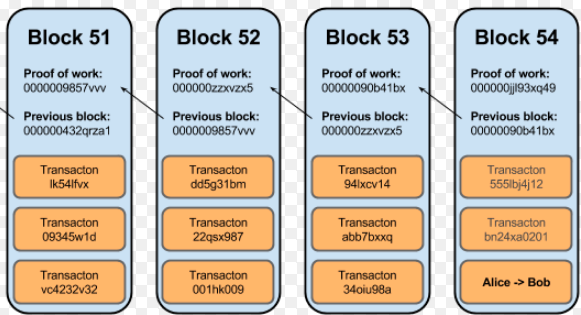
\includegraphics[width=10cm]{graphics/bitcoin-blockchain.png}
\end{center}

\end{frame}
\normalsize

%%%%%%%%%%
